\documentclass[12pt]{article}
\usepackage[english]{babel}
\usepackage[utf8x]{inputenc}
\usepackage{amsmath}
\usepackage{graphicx}
\usepackage{booktabs}
\usepackage{float}
\usepackage[colorinlistoftodos]{todonotes}
\usepackage{epstopdf}
\usepackage[margin=1.0in]{geometry}
\usepackage{hyperref}

% Source code formating
\usepackage{listings}
\lstset{ 
 %frame=single,
 language=Verilog,
 %numbers=left,
 breaklines=true,
  basicstyle=\small, %or \small or \footnotesize etc.
 title=\lstname
}


\begin{document}

\begin{titlepage}

\newcommand{\HRule}{\rule{\linewidth}{0.5mm}} % Defines a new command for the horizontal lines, change thickness here

\center % Center everything on the page


\textsc{\LARGE Harvey Mudd College}\\[1.5cm] % Name of your university/college
\textsc{\large Engineering 155}\\[0.3cm] % Minor heading such as course title
\textsc{\Large Microprocessor Systems: Design and Application}\\[0.5cm]  % Major heading such as course name

\HRule \\[0.1cm]
{ \huge \bfseries Internet-Controlled AGV}\\[0.1cm] % Title of your document
\HRule \\[1.5cm]
 

\begin{minipage}{0.4\textwidth}
\begin{flushleft} \large
\emph{Authors:}\\
Aaron \textsc{Rosen}

Alex \textsc{Rich}
\end{flushleft}
\end{minipage}
~
\begin{minipage}{0.4\textwidth}
\begin{flushright} \large
\emph{Professors:} \\
David \textsc{Harris} % Professor's Name

Matthew \textsc{Spencer}
\end{flushright}
\end{minipage}\\[1cm]



{\large December 11, 2015}\\[1cm] 


\begin{abstract}
%THIS NEEDS TO BE COMPLETED WHEN EVERYTHING IS DONE
\end{abstract}

\vfill % Fill the rest of the page with whitespace

\end{titlepage}




%\newpage
%
%{\footnotesize \tableofcontents}

\newpage


%%%%%%%%%%%%%%%%%%%%%%%%%%%%%%%%%%%%
%       INTRODUCTION
%%%%%%%%%%%%%%%%%%%%%%%%%%%%%%%%%%%%
\section{Introduction}

\begin{figure}[b!]
\begin{center}
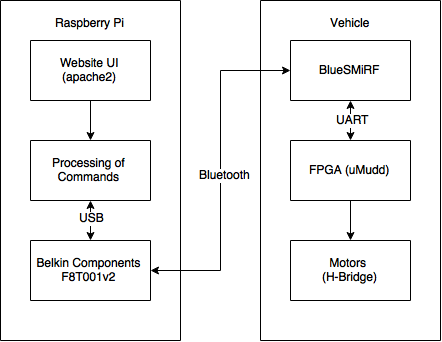
\includegraphics[width=0.7\textwidth]{E155System}
\end{center}
\caption{An overview of the system. The system is comprised of two major subsystems: the Raspberry Pi 2 controller and the vehicle, which is controlled by the $\mu$Mudd board.}
\label{fig:sys}
\end{figure}

The Internet-Controlled Autonomous Ground Vehicle is a treaded chassis that holds an FPGA with bluetooth listening capabilities. A companion website allows a user to interact with the vehicle by commanding it to travel it to various places. The motivation behind this project was to build a tank that could navigate within a map and shoot NERF darts. By building a tank that is remotely controlled over the internet, the more difficult part of this concept is realized.

The project involves a website hosted by Apache2 on the Raspberry Pi 2, which sends commands from the a bluetooth dongle to a bluetooth receiver (BlueSMiRF) that is connected to the FPGA. The FPGA drives two motors. Each component is described further in the following sections.

\section{New Hardware}
\subsection{BlueSMiRF}
\subsection{Vehicle}
\section{Schematics}

\begin{figure}
\begin{center}
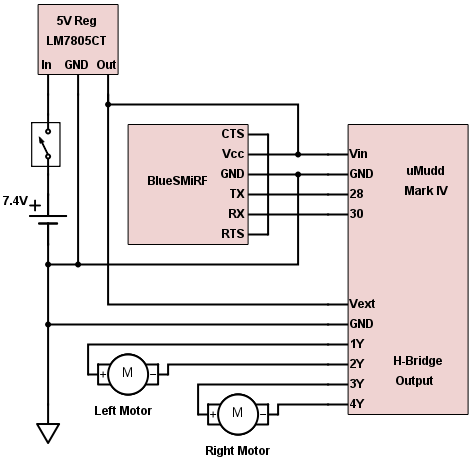
\includegraphics[width=0.7\textwidth]{breadboard}
\end{center}
\caption{The components on the breadboard. The H-Bridge Output are PWM signals.}
\label{fig:piroutines}
\end{figure}

\section{Raspberry Pi}

The Raspberry Pi 2 serves several functions. It hosts an Apache2 website accessible via the internet and contains code to submit commands to a bluetooth dongle. These two functions are integrated such that a user interacts with the website, indirectly sending commands over bluetooth. Figure \ref{fig:piroutines} show the flow of data and control through the Pi.

\begin{figure}
\begin{center}
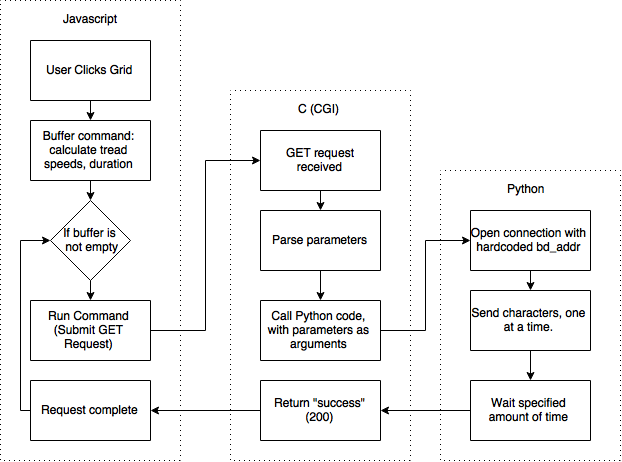
\includegraphics[width=0.8\textwidth]{PiRoutines}
\end{center}
\caption{The flow of control and data through the Pi.}
\label{fig:piroutines}
\end{figure}

\subsection{Website}

The website contains a visual user interface that contains instructions for use, a grid on which to input locations for the robot to maneuver to, a list of the commands currently buffered for sending. The code for the website is shown in Appendix A. The website was built using HTML, JavaScript, and Bootstrap CSS. 

The Pi hosts the website. Upon clicking in a grid space, the page's JavaScript calculates the left and right tread speeds and duration of movement required to get the tank to move from its original position to the new position. The current algorithm involves first moving north/south, turning, moving east/west, and finally turning to reorient itself vertically. Once the commands are generated, the JavaScript makes an HTTP GET request to the inputChars resource of the Pi. When the request is completed, the page updates, either submitting the next command in the buffer or waiting for another input from the user.

\subsection{Python/C}
After receiving a GET request, the common gateway interface (CGI) reads the input parameters (three integers) and converts them into a format that the vehicle understands. This involves converting the numbers to sign/magnitude bit representations. Because of how the UART works, the C also reverses the bits.

calls a Python script. The Python script utilizes the \verb.bluetooth. module to allow sending data using the bluetooth dongle. Since the robot has a constant bluetooth device address, this address is hard coded into the Python script. When called, the python script sends the commands, one at a time, to the robot. Currently, the system sleeps for an amount of time to theoretically give the vehicle enough time to move. However, in the future, the Pi will wait for acknowledgement from the FPGA. The code on the Pi is shown in Appendix B. 

{\it // Depending on room, I can include the code used to call Python, since that seemed to be a common problem.}

\section{FPGA Design}

The FPGA reads data from the BlueSMiRF using UART hardware coded in SystemVerilog, processes and executes the command, and then sends an acknowledgment back to the Raspberry Pi.  It is constructed as a controller-datapath pair with three main submodules in the datapath - receiveMSG, executeCommand, and sendAck.  The SystemVerilog code installed on the FPGA is shown in Appendix C. The FPGA and BlueSMiRF are the only two electrical components on the breadboard. Two motors are connected to the $\mu$Mudd board's H-bridge screw terminals.  The schematic is shown in figure.

The clock used to interface with the BlueSMiRF is implemented using a PLL that oversamples the 115.2 Kbaud UART frequency at 921.6kHz, or a factor of 8.  This oversampler determines if there is an incoming message.  The actual sampling of the BlueSMiRF's TX line is accomplished using a frequency divider that allows for sampling at the correct rate.  The divider's phase can be frozen when the start bit has not yet been detected.  This ensures that the sampling of the line is as close to the center of the transmission's clock as possible.  The Raspberry Pi sends three characters, which are flushed by the Bluetooth module's buffer at the same time, so the command appears as a 30-bit message.  The sampler stops sampling when it sees a stop bit, and either begins a new message if the next bit is a start bit, or signals to the controller that a command has been received of an entire command if the line has remained high.

The FPGA executes the command received by controlling the two motors via the H-Bridges on the $\mu$Mudd board. Each command consists of a PWM setting and rotation direction for each motor and a duration for which the motors should be turning.  A counter is used to create a reference clock for PWM; the power levels are referenced against this counter to determine the correct duty cycle.  Multiplexers are used to route the power to the correct pins on the H-Bridge, allowing for both forward and backwards movement.  To prevent the vehicle from running indefinitely, the timer stops incrementing when the requested duration is reached, and a signal is output that is used to cut power to the motors.  Each LSb of the duration character corresponds to roughly one-tenth of a second.

Once the requested duration has been reached and power to the motors cut, the FPGA transmits the character `A' back to the BlueSMiRF as an ACK code.  After this ACK has been sent, the FPGA will return to the receiveMSG state and start to sample for a new command.

A flowchart detailing each state of the FPGA is shown in Figure \ref{fig:fpgablock}.

\begin{figure}
\begin{center}
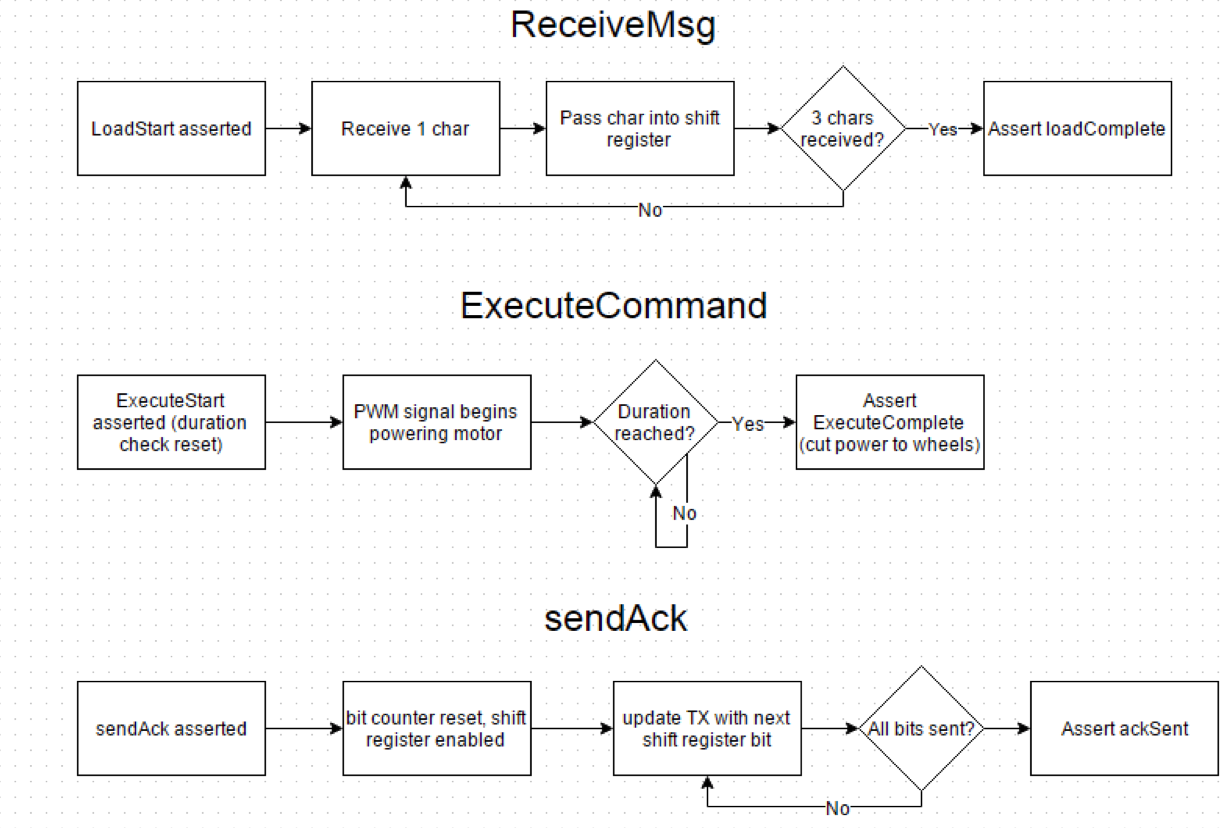
\includegraphics[width=0.8\textwidth]{FPGABlock}
\end{center}
\caption{Schematic overview of the FPGA.}
\label{fig:fpgablock}
\end{figure}

\section{Results}
\section{References}
\renewcommand{\refname}{}
\vspace{-1cm}
\begin{thebibliography}{widest entry}
 \bibitem{E102}
REFERENCES?
\end{thebibliography}
\section{Parts List}
This is the bill of materials for the project.
\begin{center}
\begin{tabular}{|l|l|l|l|}
\hline
\multicolumn{1}{|c|}{\textbf{Item}} & \multicolumn{1}{c|}{\textbf{Description}}               	& \multicolumn{1}{c|}{\textbf{Source}} & \multicolumn{1}{c|}{\textbf{Cost}} \\ \hline
Tracked Vehicle 			&										&							&	\\
			Chassis Kit	& Chassis for the tank, includes treads and frame.    	& Amazon 					& 15.39                          	\\ \hline
Tamiya 70168				& Gives tank flexibility to turn by controlling each     	& 							& \\
Double Gearbox			& tread independently.						& Amazon		               			& 11.99                             	\\ \hline
$\mu$Mudd Board                	& Controls the vehicle.                                                & E155                                 		& 0.00                               	\\ \hline
			                      	& Provides website interface and sends commands 	&							&\\
Raspberry Pi 2			    	& to vehicle.             							& E155                                 		& 0.00                               	\\ \hline
                        				& Wirelessly communicate via Bluetooth between  	&							&\\
BlueSMiRF				& Pi and $\mu$Mudd board.		 			& E155                                		& 0.00                               	\\ \hline
Belkin Components			&										&							&					\\ 
FT8001					& Send bluetooth data from Pi.					& E155                                		& 0.00                               	\\ \hline
2X TrustFire 14500			& Li Ion battery, 3.7 V 						& Aaron Rosen					& 0.00				\\ \hline
						& 										& 							& {\bf 27.38}			\\ \hline
\end{tabular}
\end{center}


\section{Appendices}
\subsection{FPGA Code}
\lstinputlisting[language=Verilog]{VehicleControl.sv}

\end{document}
